\subsection{BiGUL}
\label{sec:BiGUL}

% History, website, tutorial, community
BiGUL~\cite{PEPM2016-Ko}, short for \emph{the Bidirectional Generic Update Language}, is the current result of a long line of research on \emph{bidirectional programming}~\cite{Foster2012} predominantly performed by the programming language community.
Bidirectional programming languages typically share two main ideas in common:  (i)~the task of programming a bx can be reduced by automatically deriving one direction of synchronization from the other direction that is explicitly programmed, and (ii)~well-behavedness properties are guaranteed by providing a small set of well-behaved primitive functions, and combinators to allow bx programmers to compose complex, well-behaved bidirectional programs from these primitives.

Most bidirectional programming languages address \emph{asymmetric} consistency relations, where one of the models (the \emph{view}) is fully determined by the other model (the \emph{source}).
Instead of forward and backward synchronization, the terms \emph{put} (the source is dependent, view is master) and \emph{get} (the view is dependent, source is master) are used instead.
In this asymmetric setting, \emph{get} simplifies to a function that takes a source and produces a view, i.e., the old view is not necessary. 

As a bidirectional programming language, BiGUL is unique in the sense that it provides a programming language (primitives and combinators) for programming \emph{put} instead of \emph{get}.
Such a \emph{putback-based} bidirectional programming language has the advantage that \emph{get} can be fully derived from \emph{put} (the inverse is not true in general), for the price that \emph{put} is often more complex (and thus requires more effort to program) than \emph{get}.


\subsubsection{Classification}
A summary of the features of BiGUL according to our common feature model for bx tools is provided in the first column of table~\ref{tab:features-all-tools}.
These features will now be discussed in detail in the following.

BiGUL's architecture clearly follows a \emph{restoration-based} style, i.e., the bx programmer has the job of programming \emph{put} as \emph{fCR} and thinks in terms of how to restore the consistency of both models by comparing them and making suitable changes to the dependent model.
The exact delta between the previous and current master model is thus not of primary interest.

The main application scenario addressed by BiGUL is \emph{initial-state-based}.
Referring to figure~\ref{fig:initialStateBased}, the exact tool architecture of BiGUL is the top-left restoration-based combination of \emph{fCR} and $\mathit{hAln}$.
Specific to BiGUL, \emph{put} programs tend to be a recursive, flexible mix of intertwined ``bits and pieces'' of \emph{fCR} and $\mathit{hAln}$, rather than clearly separated functions as figure~\ref{fig:initialStateBased} appears to suggest.
A further point is that BiGUL is flexible enough to be used for other application scenarios, e.g., by encoding corrs, diags, and deltas as part of the models passed to the tool.
When programming $\mathit{hAln}$, for example, one could then access this extra information and also update it if necessary.
While this is indeed possible, it is also clear that the language was specifically designed for \emph{initial-state-based} scenarios, which is how it was also applied to solve the benchmark.

BiGUL is formally founded and was originally developed in the dependently typed programming language Agda~\cite{AFP08-Norell} so as to formally verify its well-behavedness guarantees; for practical usage a Haskell port of BiGUL is provided.\footnote{\url{http://hackage.haskell.org/package/BiGUL}}
BiGUL guarantees basic \emph{round-trip laws} for the programmed \emph{put} and automatically derived \emph{get} functions.
These laws (\emph{putget} and \emph{getput}) are closely related to correctness and hippocraticness; we refer to Ko et al.~for further details~\cite{PEPM2016-Ko}.

The underlying consistency relation is never specified explicitly when working with BiGUL.
It is \emph{implicitly} implied by the provided \emph{put} program together with the guaranteed round-trip laws, which fix the corresponding derived \emph{get} program.

BiGUL represents an interesting mix of \emph{explicit} and \emph{implicit} control over consistency restoration:  \emph{put} is explicitly programmed, while \emph{get} is automatically derived, i.e., implicitly programmed.
Well-behavedness guarantees that the derived \emph{get}, if it exists, is unique for the provided \emph{put}.

Finally, BiGUL currently only supports \emph{directed} synchronization, performed \emph{on-demand} by executing \emph{put} or \emph{get} as required.
While support for (user) interaction can be implemented as required, there is no direct support for this; BiGUL is designed more for \emph{automatic} consistency maintenance. 


\subsubsection{Benchmark solution with BiGUL}

In this section we provide a top-down, high-level, and intentionally incomplete description of the solution to the Families-to-Persons benchmark with BiGUL.
Our aim is not to explain all details, but rather to impart an intuition for the basic structure of the solution.
We refer the reader interested in further details to the BiGUL solution available on GitHub.\footnote{\url{http://bit.ly/bigul-f2p-benchmarx}}

As BiGUL only directly supports asymmetric bx, the first challenge when implementing the Families-to-Persons benchmark is to decompose the symmetric bx into two asymmetric bx.
The decomposition applied in the proposed BiGUL solution is depicted in figure~\ref{fig:bigulSolnOverview}.
Bold arrows represent functions to be programmed by the bx developer, while dashed arrows represent automatically derived functions.
%
\begin{figure}[!tbp]
    \centering
    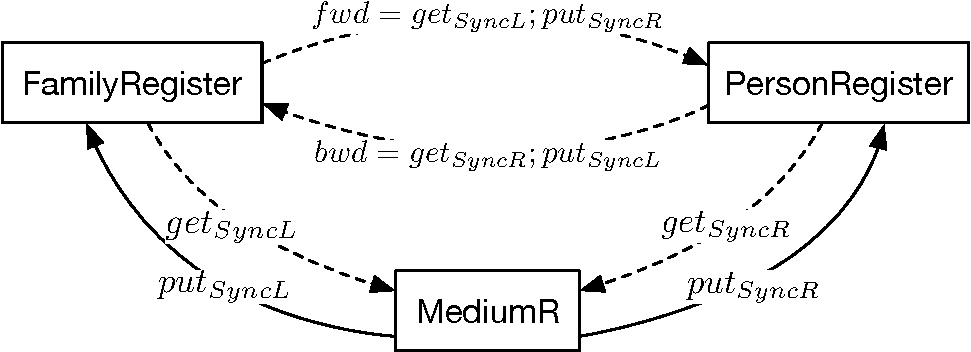
\includegraphics[width=\columnwidth]{diagrams/solutions/bigulSolnOverview}
    \caption{Handling a symmetric bx with BiGUL}
    \label{fig:bigulSolnOverview}
\end{figure}
%
In this decomposition, an additional data structure \texttt{MediumR} is introduced and can be thought of intuitively as the intersection of both data structures, i.e., it contains exactly the concepts that are present in both the source and target model spaces and that must be kept consistent.
All the bx developer now has to do is program how \texttt{MediumR} models can be \emph{put} into \texttt{Person\-Regis\-ter} models via $put_{SyncR}$, and into \texttt{Family\-Regis\-ter} models via $put_{SyncL}$.
The required \emph{fwd} and \emph{bwd} transformations can then be computed as depicted in figure~\ref{fig:bigulSolnOverview} by composing programmed \emph{put} and derived \emph{get} arrows as required.\footnote{The actual solution is a bit more complex as \emph{SyncL} is further decomposed into two arrows.}

To provide a feeling for actual BiGUL code, listing~\ref{lst:bigulSolnDetails} depicts the BiGUL program for $put_{SyncR}$.
Recall that the architecture for this solution is restoration-based (with $\mathit{hAln}$) for an initial-state-based scenario.
So this code represents \emph{fCR} and $\mathit{hAln}$ (see figure~\ref{fig:initialStateBased}).

\lstdefinelanguage{bigul}{
	morekeywords = {rearrS, Case, Skip},
	morecomment=[l]{--},
}

\begin{lstlisting}[label={lst:bigulSolnDetails}, float=htb!, language=bigul, caption={Structure of a BiGUL program}]
syncR :: BiGUL PersonRegister MediumR
syncR =
  $(rearrS [| \(PersonRegister ps) -> ps |])$
    align (const True)
      (\p (name, gender) -> 
        splitFullName 
          (getFullName p) == name &&
          isMale p == gender)
      (Case [ 
        $(normalSV 
          [p| Male _ _ |] 
          [p| _ |] 
          [p| Male _ _ |])
            ==>$(update 
                [p| Male name _ |] 
                [p| (name, True) |] 
                [d| name = Skip splitFullName |]),
        $(normalSV 
          [p| Female _ _ |] 
          [p| _ |] 
          [p| Female _ _ |])
            ==>$(update 
                [p| Female name _ |] 
                [p| (name, False) |] 
                [d| name = Skip splitFullName |])
        ])
      (\((familyName, firstName), gender) ->
          (if gender then Male else Female) 
          (familyName ++ ", " ++ firstName) 
          defaultDate)
      (const Nothing)
\end{lstlisting}

As both models are essentially lists (of persons and $(name,\- gender)$ pairs) $\mathit{hAln}$ can be implemented with the auxiliary, higher-order function \texttt{align} (line 4) that takes a matching condition and uses it to lift a BiGUL program on elements to lists.
The simple strategy is to traverse the list of view elements and to search for the first source element that matches according to the condition (here simply a comparison of name and gender on lines 7--8).
If a match is found then the first part of the \emph{fCR} code (lines 10--25) is executed (it does nothing as the elements are already consistent), if no match can be found then a new source element is created using the second part of the \emph{fCR} code (lines 27--30).
If unmatched source elements remain after all view elements have been matched, they are deleted by \texttt{align}.

Finally, although the code might appear cryptic without looking up all details, the used BiGUL primitives are highlighted as keywords in listing~\ref{lst:bigulSolnDetails}.
The point here is that the entire program is actually a composition of primitives, but is designed in a way that it appears to be written in an imperative programming language~\cite{POPL2018-Ko}.

%%% Local Variables:
%%% mode: latex
%%% TeX-master: "../main"
%%% End:
